\documentclass[11pt]{article}
\usepackage[margin=1in]{geometry}                % See geometry.pdf to learn the layout options. There are lots.
\geometry{letterpaper}                   % ... or a4paper or a5paper or ... 
%\geometry{landscape}                % Activate for for rotated page geometry
%\usepackage[parfill]{parskip}    % Activate to begin paragraphs with an empty line rather than an indent
\usepackage{color}
\definecolor{myblue}{rgb}{0.0, 0.0, 0.85}
\usepackage[breaklinks=true, colorlinks=true, linkcolor=red, urlcolor=myblue, citecolor=black]{hyperref}
\urlstyle{rm}
\usepackage{mathptmx}
\usepackage{graphicx}
\usepackage{amssymb}
\usepackage{epstopdf}
\usepackage{sidecap}
\usepackage{authblk}
\usepackage{booktabs}
\usepackage[font=small,labelfont=bf]{caption}
\usepackage{enumitem}
\usepackage{wrapfig}
\usepackage{draftwatermark}
\SetWatermarkText{DRAFT}
\SetWatermarkScale{1.2}
\SetWatermarkColor[gray]{0.85}
\DeclareGraphicsRule{.tif}{png}{.png}{`convert #1 `dirname #1`/`basename #1 .tif`.png}
\pagestyle{plain}

\def\bfr{\bf\color{red}}
\def\bfp{\color{magenta}}
\def\geohub{{\tt geohub}}
\def\resp{respectively}
\def\selah{SELAH}
\def\nch{718}
\def\nh{957\pm94}
\def\dh{10\%\pm9\%}
\def\nce{389}
\def\ne{556\pm83}
\def\de{15\%\pm12\%}

\begin{document}
%\maketitle

\begin{center}
	\Large\bf Highland Park + Eagle Rock's Unsheltered Population Is Unchanged from 2020\\
	\vspace{1ex}
	{\normalsize\rm Louis Abramson, PhD, and Brian Kohan\\ \today 
	}{\bfr \texttt{ -- NOT FOR DISTRIBUTION}}
\end{center}

\noindent {\bf Summary:} Volunteers surveying  Highland Park and Eagle Rock (HPER) on 29 April 2021 
found  a non-significant change in adults experiencing unsheltered homelessness compared to the 2020 
LAHSA Count: $-5\%\pm16\%$ (90\% CI). Declines of 20\% and 65\% in the number of identified rough 
sleepers and vans, \resp, were offset by an 87\% increase in tents and makeshift dwellings 
(Figure \ref{fig:rawCounts}). This near-doubling of the most visually salient part of unsheltered 
living would support subjective impressions that the state of homelessness worsened despite the 
total population remaining statistically unchanged. Data from the Coordinated Entry System will 
reveal how changes in sheltered homelessness affected HPER's total unhoused 
population.
%As COVID-related contractions in health, sanitation, and social 
%services, have deteriorated conditions on the street, such impressions may yet be accurate. 

\begin{table*}[h]
\caption{Unsheltered Data for Eagle Rock/Highland Park}
\resizebox{\linewidth}{!}{%
\begin{tabular}{lccccccccc}
\toprule
 & Persons & Car & Van & RV & Tent & Makeshift & {\bf 2021 Total} & {\bf 2020 Total} & {\% change*} \\ \cmidrule{1-10}
Counts & 61 & 18 & 18 & 55 & 41 & 30 & {\bf 223} & {\bf 226} & {\bf 1\%} \\
Inhabitants & 61 (16) & 29 (10) & 32 (11) & 79 (15) & 60 (14) & 51 (13) & {\bf 310 (53)} & {\bf 326} & {$\bf-5\%$ \bf(16\%)} \\
Category share & 20\% (5\%) & 9\% (3\%) & 10\% (3\%) & 25\% (5\%) & 19\% (4\%) & 16\% (4\%) & - & - & - \\ \bottomrule
\end{tabular}
}
\caption*{*Neither the raw counts nor inferred population change is statistically significant 
(parentheses denote 90\% uncertainties). No minors or families were sighted; two transition aged youth
tallied as ``Persons.''}
\label{tbl:summary}
\end{table*}

\begin{figure*}[h]
	\centering
	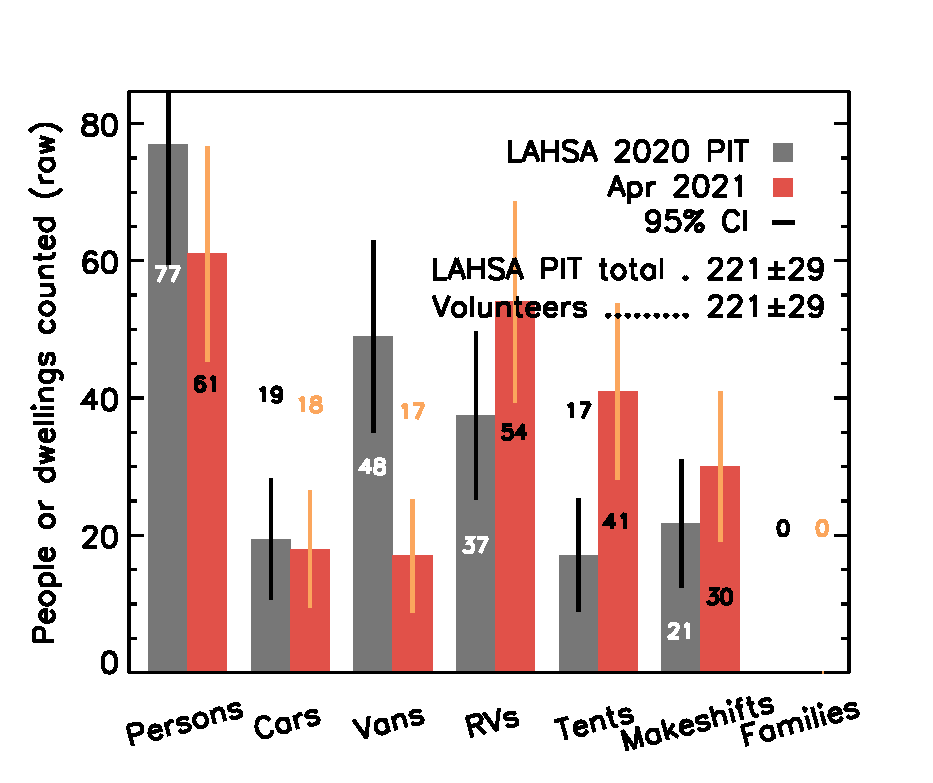
\includegraphics[width = 0.47\textwidth, trim = 1cm 0cm 0cm 1cm]{bars}
	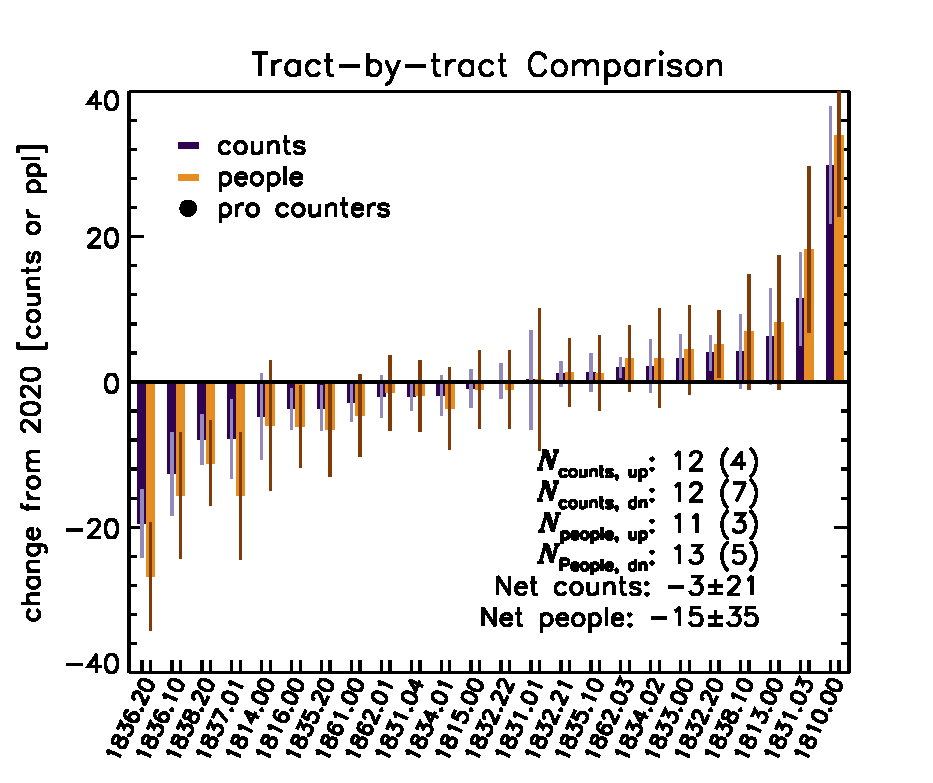
\includegraphics[width = 0.47\textwidth, trim = 0cm 0cm 0cm 1cm]{tractsYrYr.eps}	
	\caption{{\it Left:} total tallies of unsheltered persons + dwellings in Eagle Rock and
			Highland Park from the 2020 and 2021 PIT counts (grey/rust). Persons and vans 
			fell while RVs, tents, and makeshift structures rose. Overall, roughly the same number 
			of people + dwellings were identified as in 2020. {\it Right:} tract-level
			results (see also Figure \ref{fig:tcomp}, Table \ref{tbl:allTracts}). Three tracts added 
			significantly more unsheltered people, 5 lost them (parentheses
			denote significant changes). Tract 1836.20 at York/Figueroa saw the largest 
			drop ($-28$ people); 1810.00 along US 134 saw the largest gain ($+34$).}
			%``Persons'' are TAY+Adults.
	\label{fig:rawCounts}
\end{figure*}

%\pagebreak

\noindent {\bf Context:} To compensate for the 
\href{https://laist.com/latest/post/20201209/LAHSA-cancels-2021-homeless-count-los-angeles-covid-19}
{cancellation} of the annual LAHSA Count, volunteers in Highland Park and Eagle 
Rock\footnote{{\bfr ERNC, HHPNC}} conducted a grassroots vehicle-based enumeration of people 
experiencing unsheltered homelessness in those communities' 24 census tracts on April 29, 2021 
(Figure \ref{fig:tcomp}, top). Surveying ran from 7:00 PM to 11:00 PM.\\

\begin{wrapfigure}{r}{0.6\linewidth}
	\centering
	\includegraphics[width=\linewidth, trim = 0cm 0cm 0cm 0cm]{map}
	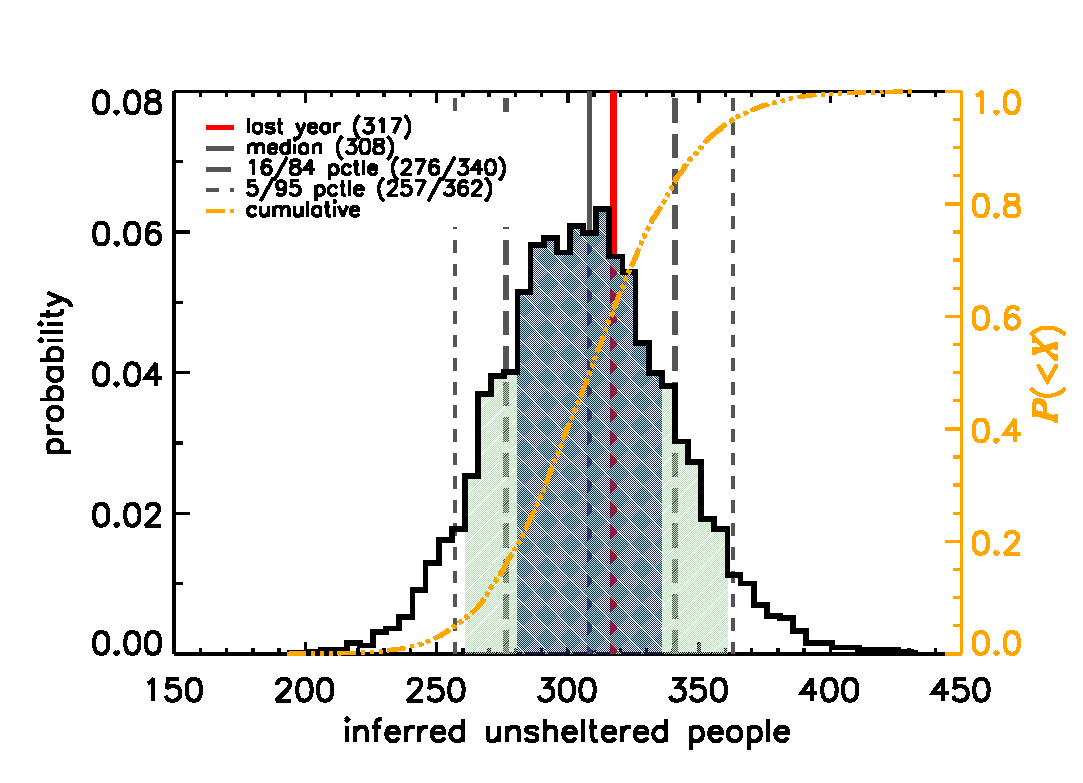
\includegraphics[width=\linewidth, trim = 0cm 0cm 0cm 0cm]{hper2021Hist}
	\caption{{\it Top:} count area with census tracts colored by  
			changes in unsheltered population from 2020 (red$+$, blue$-$).
			Tracts 1836.20 ($-28$ people) and 1810.00 ($+34$) saw the largest swings. 
			{\it Bottom:} the probability distribution for HPER's total unsheltered 
			population. The median is 5\% below 2020's value, but this change is not 
			statistically significant.
			Explore more at \href{https://pit.demoply.org}{pit.demoply.org}.}
	\label{fig:tcomp}
\end{wrapfigure} 

\noindent {\bf Results:} The population estimates in Tables \ref{tbl:summary} and \ref{tbl:allTracts} 
reflect all identified persons, cars, vans, RVs, tents, and makeshift structures with each
dwelling weighted by its average occupancy. The weights were set as the 
\href{https://www.lahsa.org/documents?id=4635-usc-2018-2020-multipliers-and-estimates-overview}
{SPA4/CD14 weights} adopted in the last official 
\href{https://www.lahsa.org/documents?id=4686-2020-greater-los-angeles-city-community-homelessness-report-service-planning-area-4.pdf}{LAHSA Community Summaries}. Results are unchanged if 
the \href{https://www.lahsa.org/documents?id=4693-2020-greater-los-angeles-homeless-count-cvrtm-conversion-factors}{SPA4-wide} occupancies are used instead, or if the tent weight is 
updated based on a survey performed by {\it SELAH}.\footnote{Outreach teams 
assessed that XX people occupied YYY surveyed tents the HPER communities,
yielding an estimated $XX\pm YY$ people per tent vs.~LAHSA's 2020 value of $1.48\pm0.11$.}

\textbf{Using Monte Carlo methods, HPER's unsheltered population is inferred to be 
310 people---16 people lower than 2020's value. However, counting and weighting uncertainties lead
to a 90\% confidence interval of $\mathbf{\pm53}$ people (Figure \ref{fig:tcomp}, bottom). The 
inferred 5\% decrease is therefore consistent with HPER's \emph{true} unsheltered population 
remaining the same as it was last year.}
%, such that 22/100 simulated surveys would have found \emph{fewer} unsheltered people compared to last year

%\begin{wrapfigure}{l}{0.625\linewidth}
%	\centering
%	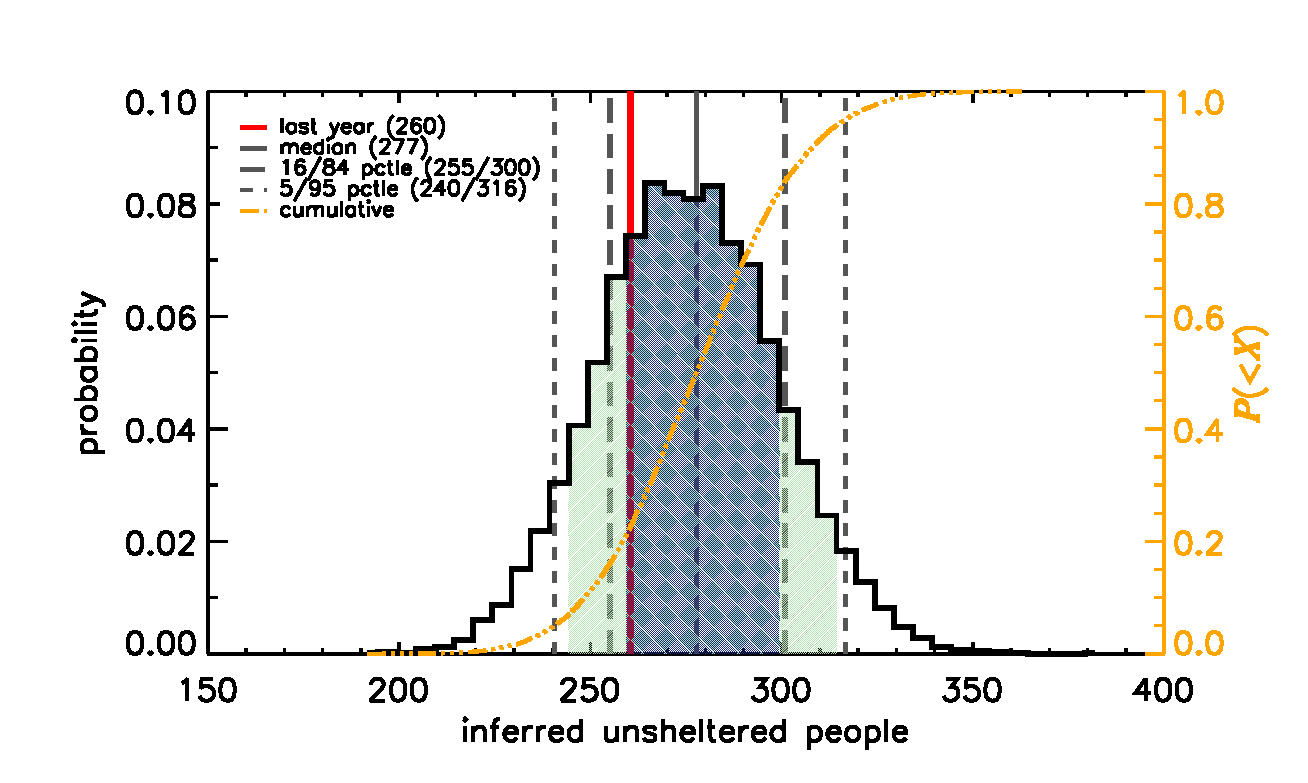
\includegraphics[width=\linewidth, trim = 0cm 0cm 0cm 0cm]{mcw2021Hist}
%	\caption{Probability distributions for the total unsheltered population in Mid City West.}
%	\label{fig:hist}
%\end{wrapfigure} 

Each of the 24 total tracts were counted once, with daytime surveys of parkland areas in two tracts
(Table \ref{tbl:allTracts}). Additionally, only the ``B'' splits were counted in two additional tracts to 
conform the survey to HPER borders as defined by LAHSA and the \href{https://statisticalatlas.com/neighborhood/California/Los-Angeles/Eagle-Rock/Overview}{Statistical Atlas}. Splits 1851.00c and 
1994.00a---which some sources affiliate with ``Highland Park''---were also not counted. The latter
of contained 32 unsheltered people in 2020. The count uncertainty is $\pm$13\% (95\% CI), 
with the remainder of the $\pm$16\% total population margin of error due to ranges in 
dwelling occupancies.\\

\noindent {\bf Comments:} The above results reflect a $\sim$20\% drop in the number
of adult individuals seen on the street---mirroring trends in 
\href{https://www.latimes.com/homeless-housing/story/2021-04-13/despite-appearances-15-fewer-homeless-people-were-on-hollywood-streets-this-year}{Hollywood} and Mid City West---combined with a {\bf 65\% 
drop in identified van dwellings}, and offset by an {\bf 87\% increase in tents and makeshift structures}. 
Government initiatives to stop evictions and move people off the streets may be responsible. 
If \href{https://www.lahsa.org/documents?id=4673-2020-homeless-count-council-district-14}{CD14's} 11\% share of \href{https://www.lahsa.org/documents?id=4585-2020-greater-los-angeles-homeless-count-los-angeles-continuum-of-care-coc-}{LA County's unsheltered seniors} 
is an indication, 200 CD14 residents might have been in any of Project Roomkey's 
\href{https://projectroomkeytracker.com/}{1826 active rooms} on the night of the count, including 
those in {\bfr known shelters}.\footnote{Due to the presence of Skid Row, CD14-level trends may not
reflect those in HPER.} {\bfr New Safe Parking responsible for the van decline? But it's not seen in cars.}
Coordinated Entry System data will show if the above scenarios are true.

\begin{wraptable}{r}{0.55\linewidth}
\caption{Eagle Rock/Highland Park Tract-level Unsheltered Data}
\resizebox{\linewidth}{!}{%
\begin{tabular}{cccccc}
\toprule
Tract & Counter & Passes & Median Est. & 90\% CI \\ \cmidrule{1-5}
1810.00$^{\rm a}$ & V & 1 & 59 & 44--74 \\
1813.00 & V & 1 & 33 & 22--45 \\
1814.00 & V & 1 & 21 & 10--31 \\
1815.00 & V & 1 & 4 & 0--11 \\
1816.00$^{\rm a}$ & V & 1 & 2 & 0--9 \\
1831.01 & V & 1 & 31 & 19--43 \\
1831.03 & V & 1 & 40 & 25--58 \\
1831.04 & V & 1 & 1 & 0--8 \\
1832.20 & V & 1 & 6 & 0--13 \\
1832.21 & V & 1 & 3 & 0--10 \\
1832.22 & V & 1 & 4 & 0--11 \\
1833.00 & V & 1 & 11 & 1--19 \\
1834.01 & V & 1 & 4 & 0--11 \\
1834.02 & V & 1 & 12 & 3--22 \\
1835.10 & V & 1 & 6 & 0--13 \\
1835.20 & V & 1 & 5 & 0--13 \\
1836.10 & V & 1 & 15 & 5--24 \\
1836.20 & V & 1 & 1 & 0--8 \\
1837.01 & V & 1 & 15 & 6--23 \\
1838.10 & V & 1 & 22 & 11--32 \\
1838.20 & V & 1 & 3 & 0--10 \\
1861.00$^{\rm b}$ & V & 1 & 3 & 0--10 \\
1862.01 & V & 1 & 4 & 0--11 \\
1862.03$^{\rm b}$ & V & 1 & 3 & 0--10 \\
\cmidrule{1-5}
{\bf All} & &{\bf 24} & {\bf 310} & {\bf 250--366}
\\ \bottomrule
\end{tabular}
}
\caption*{$^{\rm a}$ Rec center surveyed on foot circa 3:00 PM; $^{\rm b}$ ``Split B'' only.}
\label{tbl:allTracts}
\end{wraptable} 

While the number of people on the street may be unchanged, their quality of life has worsened. 
COVID has restricted or eliminated access to restaurant bathrooms, libraries 
(\href{https://www.lapl.org/homeless-resources/the-source}{\it The Source}), DPSS 
(EBT, Medi-Cal), DMV (IDs), and DMH facilities. Physical limits on client access at 
hospitals has also kept caseworkers from managing successful discharges. These harms 
are reflected by a 33\% increase in 
\href{http://publichealth.lacounty.gov/chie/reports/HomelessMortality2020_CHIEBrief_Final.pdf}{overdose deaths} and made more visible by \href{https://clkrep.lacity.org/onlinedocs/2020/20-0147_misc_3-17-20_p.pdf}{suspended}
tent folding and sanitation practices as tents increased.
Of course, with no drop observed with them in place, a substantial rise in unsheltered homelessness
is likely \href{https://www.latimes.com/california/story/2021-01-12/new-report-foresees-tens-of-thousands-losing-homes-by-2023}{once the eviction moratoria lapse}.

The data support the effectiveness of programs aimed at curbing a rise in street homelessness.
Yet, they do {\it not} suggest that the state of homelessness has improved. In the fight to rebuild 
lives as we build homes, that fact must remain paramount.

%\clearpage

\end{document}  